\chapter{Security of an encryption protocol}\label{chap:security}
In this chapter, we give the formal definition of security of symmetric encryption and test our developed Rubik's Cube encryption protocol against it. We make essential tweaks to the Rubik's Cube encryption to make it fit in the definition, and we generate some statistics to show that the final improved encryption produces a good shuffling.

\section{What is security?}
We denote the Rubik's Cube encryption protocol as $\Pi_{RC} = (\textbf{Gen}, \textbf{Enc}, \textbf{Dec})$. Let us first review procedures of $\Pi_{RC}$ by listing out details of each component, assuming that we are still using a normal 3 by 3 by 3 cube.
\begin{itemize}
    \item \textbf{Gen} takes an integer $n$ as input representing the number of fundamental moves in the key. It then draws one move from the 18 fundamental moves uniformly at random $n$ times and denotes the series of moves as $k$. Afterwards, it picks one permutation from $S_{216}$, the permutation group on 216 elements, uniformly at random and denotes the permutation as $p$. Finally, \textbf{Gen} outputs $(k, p)$.
    
    \item \textbf{Enc} takes a tuple $(k, p, m)$, where $m$ has length of 216 bits, as the input. Then it fills an empty cube with $m$ in the following order: top face $\rightarrow$ front face $\rightarrow$ right face $\rightarrow$ down face $\rightarrow$ back face $\rightarrow$ left face. Recall Figure~\ref{fig:bit-order}, for each face, \textbf{Enc} starts to fill at the left up corner cubie, and once it completes a row, it goes to the next row until it reaches the right down corner cubie. For each cubie, \textbf{Enc} fills it with the order: left up corner $\rightarrow$ right up corner $\rightarrow$ right down corner $\rightarrow$ left down corner. After filling the cube, \textbf{Enc} permutes the bits on the cube using $p$ and applies the first movement in $k$ to the cube. Then \textbf{Enc} permutes the bits again using $p$ and applies the second movement in $k$ to the cube. \textbf{Enc} repeats itself until it reaches the last move in $k$. Finally, \textbf{Enc} reads out the bits the same order as they were put in and outputs the encrypted bits $c$. We denote this process by \textbf{Enc}$_{kp}(m)$.
    
    \item \textbf{Dec} takes a tuple $(k, p, c)$ where $c$ has length of 216 bits, as the input. It then fills an empty cube with $c$ the same way as \textbf{Enc}. Then \textbf{Dec} finds inverses of $k$ and $p$ and denotes them as $k'$ and $p'$. Afterward, \textbf{Dec} applies the first movement in $k'$ to the cube and permutes the bits on the cube using $p'$. \textbf{Dec} repeats itself until it reaches the last move in $k'$ and completes last permutation using $p'$. Finally, \textbf{Dec} reads out the bits the same order as they were put in and outputs the decrypted bits $m$. We denote this process by \textbf{Dec}$_{kp}(c)$.
\end{itemize}
In the last chapter, we claimed our improvements would make the encryption scheme stronger against the brute force attacks. However, does that mean we can conclude that the Rubik's Cube encryption is secure? So far, we have not yet defined what we mean by the security of an encryption protocol. Ideally, a safe encryption protocol will leak zero bit of information of the plaintext.Though this sounds like a stringent requirement, it is necessary for any secure encryption protocol to satisfy in real life applications. Suppose we are voting anonymously to select the class president between two candidates. If the encryption system we use leaks information about one letter in the plaintext and if that letter happens to exist in one candidate's name but not the other, people who monitor the Internet will then be able to tell our decisions. However, as one can imagine, deciding the amount of information leaked can be a difficult task.
\par We do so for an encryption protocol $\Pi = (\textbf{Gen}, \textbf{Enc}, \textbf{Dec})$ by defining an interactive experiment $E_{\Pi}$ between Alice, the adversary and Bob, the holder of $\Pi$.
\begin{table}[ht]
    \centering
    \begin{tabular}{|p{6.5cm}p{0.5cm}p{6.5cm}|}
        \hline \multicolumn{1}{|c}{Alice} & \multicolumn{1}{c}{|} & \multicolumn{1}{c|}{Bob} \\ \hline
        \hline Generates messages $m_0, m_1$, both of length $n$ that can be accepted by $\Pi$. Sends $m_0, m_1$ to Bob. & & \\
        \multicolumn{3}{|c|}{$\xrightarrow{\hspace{0.5cm} m_0, m_1 \hspace{0.5cm}}$} \\
        & & 
        \begin{itemize}
            \item Randomly selects $m_0$ or $m_1$.
            \item Uses \textbf{Gen} to generate a key $k$.
            \item Encrypts the selected message using $k$ to form the \textit{challenge ciphertext} $c$.
            \item Sends $c$ to Alice.
        \end{itemize} \\
        \multicolumn{3}{|c|}{$\xleftarrow{\hspace{0.9cm} c \hspace{0.9cm}}$} \\
        Guesses whether Bob encrypted $m_0$ or $m_1$ to form $c$. & & \\
        \hline
    \end{tabular}
    \caption{Procedure of experiment $E_{\Pi}$}
    \label{tab:security-experiment}
\end{table}
The details of $E_{\Pi}$ is shown in Table~\ref{tab:security-experiment}. If Alice guesses correctly on which message was encrypted, we say that Alice wins the experiment.
\par Notice that in above experiment, Alice has the freedom to pick any $m_0$ and $m_1$ as long as both of them have the desired length. Therefore, if $\Pi$ is not secure and leaks information when given certain inputs, Alice can always choose those inputs and win this experiment with a pretty good chance. However, if $\Pi$ is truly secure, in each run of the experiment, Alice has to randomly guess which message was encrypted. Therefore when $\Pi$ is secure, Alice should have exactly $\frac{1}{2}$ probability of winning the experiment $E_{\Pi}$. We now can give the formal definition of security of private-key encryption schemes.
\begin{definition}\label{def:security} \textbf{Security of private-key encryption scheme} \\
    A private-key encryption scheme $\Pi = \normalfont (\textbf{Gen}, \textbf{Enc}, \textbf{Dec})$ is secure, if for all adversaries, they have exactly $\frac{1}{2}$ chance to win the experiment $E_{\Pi}$.
\end{definition}
\par In real life, we only consider adversaries running in limited time, and therefore we allow the adversary to win with probability negligibly better than $\frac{1}{2}$. While not diving into details of negligible functions, we can solely consider it as a tiny error term.

\section{Security of Rubik's Cube encryption}
Our encryption system $\Pi_{RC}$ is not secure under Definition~\ref{def:security}. We can slightly modify Alice's strategy to show how she can always win the experiment $E_{\Pi_{RC}}$. The behavior of Alice is altered as shown in Table~\ref{tab:cube-security-experiment}.
\begin{table}[ht]
    \centering
    \begin{tabular}{|p{6.5cm}p{0.5cm}p{6.5cm}|}
        \hline \multicolumn{1}{|c}{Alice} & \multicolumn{1}{c}{|} & \multicolumn{1}{c|}{Bob} \\ \hline
        \hline Sends messages $m_0, m_1$ with $m_0 = \underbrace{000...0}_{216}$ and $m_1 = \underbrace{111...1}_{216}$ to Bob. & & \\
        \multicolumn{3}{|c|}{$\xrightarrow{\hspace{0.5cm} m_0, m_1 \hspace{0.5cm}}$} \\
        & & Same steps as in Table~\ref{tab:security-experiment}. \\
        \multicolumn{3}{|c|}{$\xleftarrow{\hspace{0.9cm} c \hspace{0.9cm}}$} \\
        Guesses $m_0$ was encrypted if $c$ is an all-zero string and guesses $m_1$ was encrypted if $c$ is an all-one string. & & \\
        \hline
    \end{tabular}
    \caption{Procedure of experiment $E_{\Pi_{RC}}$}
    \label{tab:cube-security-experiment}
\end{table}
The reason our improved encryption system quickly failed the definition of security is that it solely offers a way to permute the plaintexts without modifying any of the bits. We see that the challenger cipher $c$ must be either an all zero string or an all one string because $\Pi_{RC}$ only permutes the plaintext. Hence, by using the strategy described in Table~\ref{tab:cube-security-experiment}, Alice can win the experiment with a probability of 1. When interacting with the encryption protocol, Alice, can always find the message encrypted by merely counting the number of zeros and ones in the messages. 
\par One way for us to make further modifications to provide more security under this definition is to bring in some randomness in the encryption procedure. Intuitively, instead of using all six faces of the Rubik's Cube to hold plaintext, we use only five faces for the actual plaintext and we use one face to hold some random bits. That means instead of encrypting 216 bits, we encrypt $36 \cdot 5 = 180$ bits at a time. Suppose we use the top face, front face, right face, down face and back face for the actual message.
\begin{table}[ht]
    \centering
    \begin{tabular}{|p{6.5cm}p{0.5cm}p{6.5cm}|}
        \hline \multicolumn{1}{|c}{Alice} & \multicolumn{1}{c}{|} & \multicolumn{1}{c|}{Bob} \\ \hline
        \hline Sends messages $m_0, m_1$ with $m_0 = \underbrace{000...0}_{180}$ and $m_1 = \underbrace{111...1}_{180}$ to Bob. & & \\
        \multicolumn{3}{|c|}{$\xrightarrow{\hspace{0.5cm} m_0, m_1 \hspace{0.5cm}}$} \\
        & & Same steps as in Table~\ref{tab:security-experiment}. \\
        \multicolumn{3}{|c|}{$\xleftarrow{\hspace{0.9cm} c \hspace{0.9cm}}$} \\
        Guesses $m_0$ was encrypted if $c$ has more or equal to 180 zeros and guesses $m_1$ was encrypted if $c$ has more or equal to 180 ones. & & \\
        \hline
    \end{tabular}
    \caption{Procedure of experiment $E_{\Pi_{RC}}$}
    \label{tab:improved-cube-security-experiment}
\end{table}
We then can use the left face for the random bits. However, solely doing this will not be enough. As shown in Table~\ref{tab:improved-cube-security-experiment}, we can again modify Alice's strategy and show how she can break this improved schema. 
\par For an input with all ones, the output will have a minimum of 180 ones and the all-zero input will have a maximum of 36 ones. Therefore the adversary can still distinguish the two input messages by simply counting the number of ones and zeros.
\par Thus, to fully utilize the randomness, we want to spread it across the cube during the encryption. We can achieve such task by performing XOR operation between the left face, which holds the random bits and the rest of the faces. To make the randomness spread evenly, we want to perform this XOR operation every time before we apply the permutation and the movement to the cube. In Table~\ref{tab:xor-example}, we display the first five bits of each cube face and build a minimum example to illustrate this process. Notice that the bits on the left face remain unchanged.
\begin{table}[ht]
    \centering
    \begin{tabular}{|c|c|c|}
        \hline Cube face & Before XOR & After XOR \\
        \hline Up face & 00000... & 11111... \\
        \hline Front face & 00001... & 11110... \\
        \hline Right face & 00011... & 11100... \\
        \hline Down face & 00111... & 11000... \\
        \hline Back face & 01111... & 10000... \\
        \hline Left face & 11111... & 11111... \\
        \hline
    \end{tabular}
    \caption{Example of XOR operation}
    \label{tab:xor-example}
\end{table}
We can encrypt Einstein's quote again with the revised Rubik's Cube encryption. We need to first cut the size of the input down to 180 bits and we need to generate 36 continuous random bits.
\newpage
\begin{center}
    010001000100111101001110010011110101010001010111010011110101001001010010
    010110010100000101000010010011110101010101010100010110010100111101010101
    010100100100010001001001010001100100\textcolor{blue}{000000010111001010010100010111100010}
\end{center}
As displayed above, the leading bits are the actual input and the random bits are colored in blue. We again use the same key ``$R\,U\,B2\,L'\,D2\,F\,R'\,D\,B\,L2\,$'' to encrypt the cube. Each time before we apply one move to the cube, we first perform the XOR operation and then shift the bits. After we use all moves in the key, we get the result:
\begin{center}
    011000111101111110000110111000010010101011101011001000011101111011000100
    011010011110110101000110111101001010011101100001110001100000101011111001
    001110101110010001010011100001100011110101011101010110011000001010100000
\end{center}
Along with the random bits, the plaintext has 122 zeros and 94 ones but after the encryption, the ciphertext has 107 zeros and 109 ones. In this example, we find the number of ones and zeros become pretty balanced. If the XOR operation has the same effect on balancing the bits for all input strings, the counting method Alice can use as strategy in the experiment $\Pi_{RC}$ will become much less feasible.

\section{Analysis of Rubik's Cube encryption}
\par The implementation of the Rubik's Cube encryption system in python is attached in the Appendix. In order to illustrate some insights of how well this encryption can shuffle the input bits, we use it to generate some statistics. Also, by looking at those results, we are able to make some suggestions for picking keys with the proper length.
\par The first interesting thing we can keep track of is how bits travel when we apply a random key on the cube. Recall the order of putting the bits in by faces is: up face $\rightarrow$ front face $\rightarrow$ right face $\rightarrow$ down face $\rightarrow$ back face $\rightarrow$ left face. Each face holds 36 bits as displayed in Figure~\ref{fig:bit-order}. Thus the bits on up face will be labeled from 1 to 36, the bits on front face will be labeled from 37 to 72 and so on. Therefore we use number 1 through 216 to represent locations of all bits.
\par In Figure~\ref{fig:bits-travel}, we display how two adjacent bits at location 1 and location 2 travel under 20 random fundamental moves. Notice that, in the experiment, we used the bit shift as the permutation. 
\begin{figure}[ht]
    \centering
    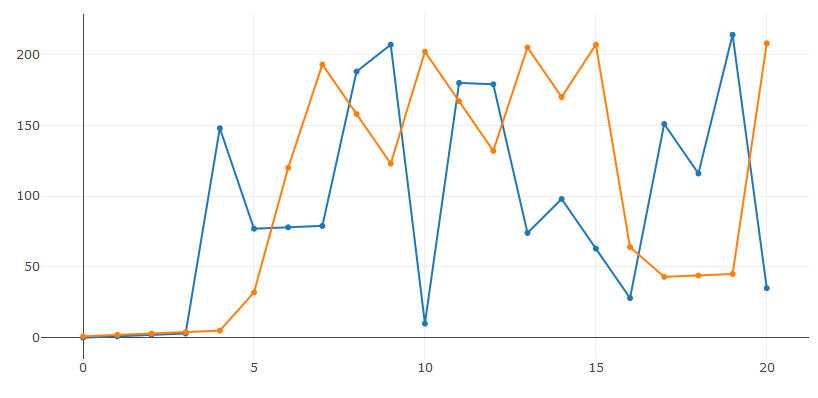
\includegraphics[width=12cm]{figures/security/bits_travel.png}
    \caption{Bit locations}
    \label{fig:bits-travel}
\end{figure}
The blue line in the graph tracks the bit at location 1 while the orange line in the graph tracks the bit at location 2. The x-axis in the graph represents the number of movements and the y-axis represents the location. These two bits end up at location 35 and location 208 individually. Though they start to be 1 space part, they end up being 173 spaces apart. We stimulated this process with 100 random series of 20 fundamental moves. Each time we recorded the final distance between the same two bits and denote the value as $FD$. Among the 100 distances $FD$ we collected, 73 were unique and the average of $FD$ is about 71 spaces. To determine the proper key length, we repeat the process by picking 100 random series for each key length and the results are displayed in Table~\ref{tab:bits-location}.
\begin{table}[ht]
    \centering
    \begin{tabular}{|c|c|c|c|c|c|}
        \hline Key length & Mean $FD$ & Median $FD$ & Max $FD$ & Min $FD$ & Unique $FD$ \\
        \hline 8 & 56.2 & 43.5 & 198 & 1 & 61\% \\
        \hline 9 & 58.8 & 47 & 194 & 1 & 63\% \\
        \hline 10 & 60.4 & 51 & 200 & 1 & 66\% \\
        \hline 12 & 66.7 & 55.5 & 212 & 1 & 68\% \\
        \hline 15 & 68.7 & 60 & 214 & 1 & 70\% \\
        \hline 20 & 70.6 & 63 & 208 & 1 & 73\% \\
        \hline 30 & 73.3 & 65 & 207 & 1 & 76\% \\ \hline
    \end{tabular}
    \caption{Statistics on $FD$}
    \label{tab:bits-location}
\end{table}
It seems that mean of $FD$, median of $FD$ and number of unique $FD$ has a positive relationship with the key length, but as key length gets longer, those values increase slower. Also we notice that even if we shuffle the cube more, two adjacent bits can still end up to be adjacent. But more fundamental moves do provide more possible final distances. As expected, we suggest using a key with longer length in general provides more security. We will discuss more in the next a couple of paragraphs to find an exact number as the suggested value.
\par In addition, we can check how the ciphertext differs from the plaintext. That is, we want to know if the XOR step does a good job mixing the zeros and ones. Let us revisit the vulnerability we found earlier. Suppose we have an all-zero string input and the bits on the left face are randomly generated. Each time we apply a random key formed by 10 fundamental moves to the cube and find the number of zeros we end up having in the ciphertext. Let us denote this value as $NZ$, short for number of zeros. We find the average of $NZ$ is about 101 when we use 10 fundamental moves. We can increase this number to see how many moves we need to make about half of the bits to be ones in the ciphertext.
\begin{table}[ht]
    \centering
    \begin{tabular}{|c|c|c|c|c|c|}
        \hline Key length & Mean $NZ$ & Median $NZ$ & Max $NZ$ & Min $NZ$ & $NZ \leq 108$ \\
        \hline 10 & 100.7 & 102 & 124 & 56 & 23 \\
        \hline 15 & 105.1 & 105.5 & 126 & 80 & 41 \\
        \hline 20 & 107.4 & 108 & 125 & 91 & 51 \\
        \hline 25 & 108.3 & 107 & 126 & 91 & 52 \\
        \hline 30 & 108.5 & 109 & 127 & 93 & 57 \\ \hline
    \end{tabular}
    \caption{Statistics on $NZ$}
    \label{tab:number-zeros}
\end{table}
From Table~\ref{tab:number-zeros}, we find that when we increase the key length to 25 fundamental moves, the average of $NA$ increases to 108.3. In addition, there were actually equal number of zeros and ones or more ones than zeros in 52 times among the 100 runs. This result provides evidence that the XOR operation can successfully hide the fact that an all zero string was encrypted. Results above suggest that a key with length of 25 fundamental moves may give us reasonable security and efficiency for the Rubik's Cube encryption.
\par Notice that if the random bits happen to be all zeros while we are inputting an all-zero string, the entire string will stay as all zeros no matter how we shuffle it. In the experiment, Alice can use this vulnerability to attack the improved encryption protocol. However, there are in total $2^{4 \cdot 3 \cdot 3} = 2^{36}$ set of bits the left face of $C_3$ can generate and only one set among those contains all zeros. If we use an arbitrary large cube $C_n$, the left face of $C_n$ can generate $2^{4n^2}$ different set of bits. Hence, Alice has a really small chance to win even if she knows about this vulnerability. We claim that Alice has merely a negligible chance to win the experiment more than half times by using the bit counting strategy.
\par One other thing that is commonly measured to test encryption protocols is called \textit{diffusion}, which means that if we flip a single bit of the plaintext and encrypt it again, then statistically, half of the bits in the ciphertext should change. We fix a random key with length of 25 fundamental moves and we create two messages that differ at exactly one bit. We encrypt both message and count how many bits between them are different. Let us denote this value as $BD$, shorten for bit difference. Similar to above, we repeat this process 100 times for each unique key lengths.
\begin{table}[ht]
    \centering
    \begin{tabular}{|c|c|c|c|c|}
        \hline Key length & Mean $BD$ & Median $BD$ & Max $BD$ & Min $BD$ \\
        \hline 25 & 70.6 & 87 & 120 & 1 \\
        \hline 30 & 79.4 & 95.5 & 123 & 1 \\
        \hline 40 & 93.2 & 104 & 122 & 1 \\
        \hline 50 & 98.2 & 108 & 125 & 1 \\ \hline
    \end{tabular}
    \caption{Statistics on $BD$}
    \label{tab:bit-difference}
\end{table}
From Table~\ref{tab:bit-difference}, we see that to provide sufficient diffusion, we need the key length to be about 50.
\par In this chapter we have introduced the formal definition of security of encryption protocols. To make the Rubik's Cube encryption stronger under this definition, we introduced randomness in the encryption procedure. We also found evidence that key length of 30 may give reasonable security and efficiency for the encryption.
\par In next chapter, we will explain some known results about the size the group $G_n$ and the explicit structure of $G_3$. This will lay the ground work for using Rubik's Cube as the basis for a key exchange system in Chapter~\ref{chap:exchange}.